While the Segment Anything Model (SAM) has demonstrated remarkable zero-shot generalization in the computer vision domain, its application to meteorological data presents two fundamental challenges. First, SAM is inherently designed for three-channel RGB images, whereas climate data, such as the ClimateNet dataset, consists of multi-parameter atmospheric grids. Unlike natural images, these variables lack high-frequency edges and clear semantic boundaries, making the standard image encoder less effective at capturing the underlying geophysical features.

Second, the operational utility of SAM is limited by its reliance on manual geometric prompts (points, boxes, or masks) to guide segmentation. In a real-time meteorological forecasting context, requiring a human expert to provide manual prompts for every global raster is impractical. Therefore, our objective is to transition SAM toward a prompt-free architecture capable of autonomous detection.

To achieve a prompt-free system that remains grounded in the physical realities of the dataset, we divide our approach into two distinct phases, as illustrated in Figure \ref{fig:pipeline}. In the Adaptation Phase, we experiment with a learnable token-based approach, inspired by HQ-SAM \cite{ke2023segment} and CAT-SAM-T \cite{xiao2024cat}, as well as a LoRA-based approach, inspired by LoRA-SAM \cite{zhang2024improving}. In the Prompt Generation Phase, we first use a pretrained CGNet from ClimateNet to produce auxiliary masks. We also experiment with a multi-scale fusion module, inspired by Self-Prompt SAM \cite{xie2025self}.

% \begin{figure}[!h]
%     \centering
%     \includegraphics[width=0.8\textwidth]{graphics/approach/approach_pipeline.pdf}
%     \caption{Pipeline}
%     \label{fig:pipeline}
% \end{figure}

\begin{figure}[!h]
    \centering
    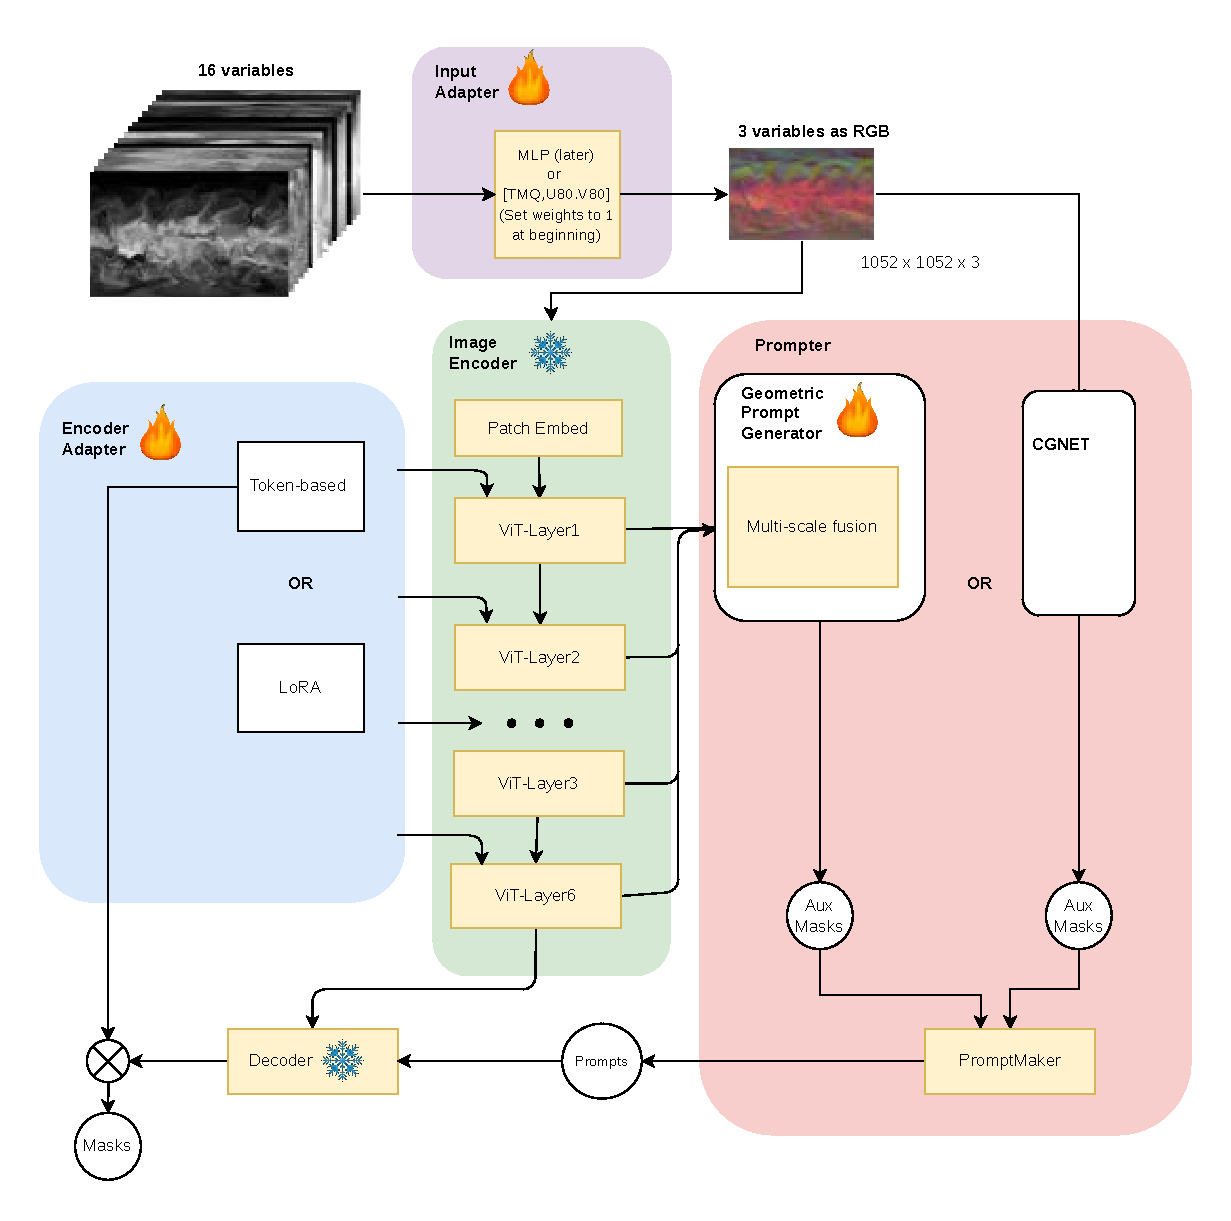
\includegraphics[width=1\textwidth]{graphics/approach/pipeline.pdf}
    \caption{Experiment Pipeline}
    \label{fig:pipeline}
\end{figure}

\subsubsection{Phase 1: Adaptation and Encoder Refinement}

The primary objective of the first phase is to enable the SAM  to interpret non-image atmospheric variables, which differ significantly from the RGB data for which the model was originally optimized. To bridge the structural gap between the 16 multi-channel atmospheric grids  and the fixed input requirements of the SAM image encoder, we implement a dual adaptation strategy:

\begin{enumerate}
\item Learnable Token-based Adaptation: We introduce learnable tokens to compress the high-dimensional atmospheric channels into a latent representation that aligns with the encoder's expected feature space.
\item Low-Rank Adaptation (LoRA): To maintain the foundational knowledge of the pre-trained model while specializing it for meteorological features, we utilize LoRA to fine-tune specific layers within the encoder and mask decoder.
\end{enumerate}


During this stage, the model is trained under the assumption of ``perfect prompts". By providing the system with ground-truth bounding boxes or point coordinates during the training phase , we isolate the adaptation process of the encoder and the mask decoder. This methodology ensures that the model focuses exclusively on learning to extract high-quality, diagnostic features from critical variables.

By removing the variability of prompt quality, we can more accurately evaluate the model's ability to handle the ``ribbon-like" structures of Atmospheric Rivers (ARs) and the circular patterns of Tropical Cyclones (TCs) , effectively mitigating the challenges posed by data imbalance and the lack of traditional image-style boundaries.

\subsubsection{Phase 2: Automated Prompt Generation}
Once the encoder is successfully adapted to the ClimateNet domain, we introduce a generator module to eliminate the need for manual intervention. This generator leverages the embeddings produced by the encoder to automatically predict the locations of TCs and ARs. By treating the image embeddings as a rich source of contextual information, the generator produces auxiliary segmentation masks. These masks are then processed to generate point and bounding box prompts, which are fed into the mask decoder to produce the final segmentation for evaluation.

\section{Dataset Preparation}
% Here I would write how the data from sources, z-normalize, make it images again by multiply by 255. 
% How prompts is make, take the multimask ground truth, find connected component, filter out, get N positive points, or M negative points per object masks, bounding box, noisy mask (resize, iroduce noise, 

The Figure \ref{fig:prompt_pipeline} illustrates the overall pipeline of prompt preparation for GAN. This includes creating point prompts, bounding box prompts, and noisy mask prompts for the input adapter in phase 1 as well as creating prompts from auxiliary masks from automatic prompt generator from phase 3.

\begin{figure}[!h]
    \centering
    % 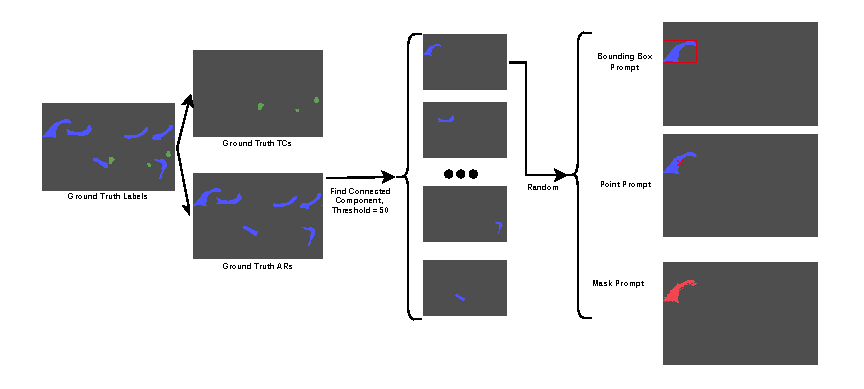
\includegraphics[width=1\textwidth]{graphics/approach/prompt_pipeline-1.pdf}
    \makebox[\textwidth][c]{%
    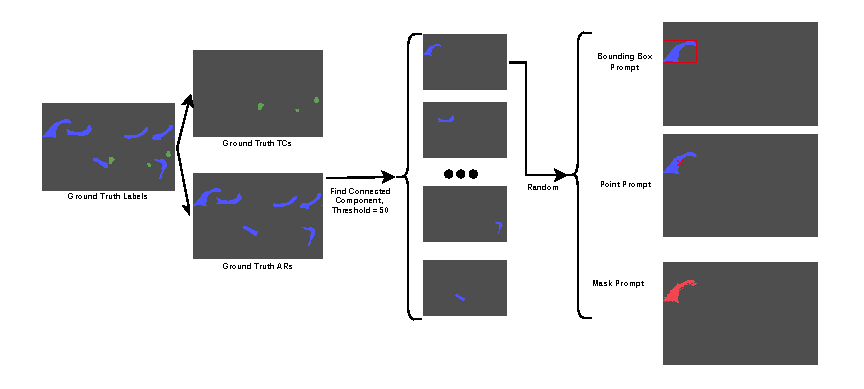
\includegraphics[width=1.2\textwidth]{graphics/approach/prompt_pipeline-1.pdf}
}
    \caption{Prompt Preparation Process}
    \label{fig:prompt_pipeline}
\end{figure}

The Figure \ref{fig:point_prompt_generation} and \ref{fig:noisy_mask_generation} describe the process of creating point prompts and noisy mask prompts in detail. To generate positive point prompts, the binary mask is first processed using an erosion operation with a kernel size determined by the object area. Positive points are then randomly sampled from this eroded region, ensuring the points remain well within the object boundaries. For negative point prompts, the pipeline utilizes two different dilation kernels. A smaller kernel and a big kernel are applied to the mask, and the smaller dilated version is subtracted from the larger one to define a boundary region for sampling negative points. 

\vspace{-2em}
\begin{figure}[!h]
    \centering
    % 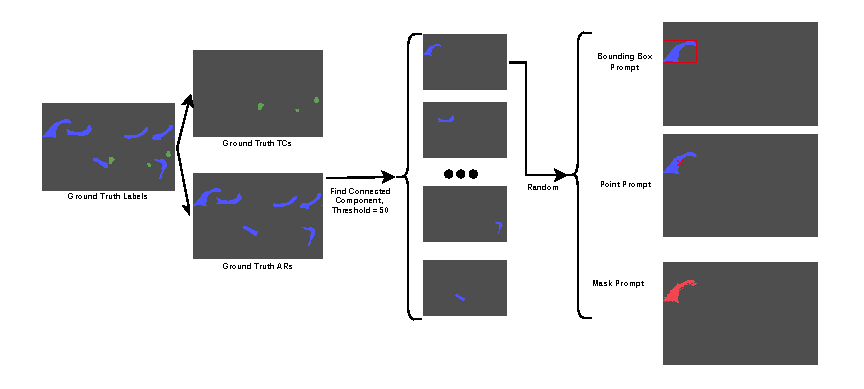
\includegraphics[width=1\textwidth]{graphics/approach/prompt_pipeline-1.pdf}
    \makebox[\textwidth][c]{%
    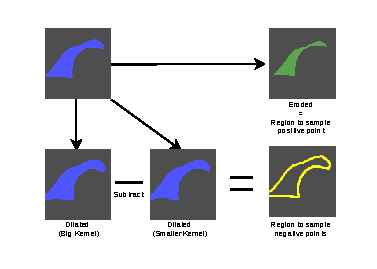
\includegraphics[width=0.7\textwidth]{graphics/approach/point_prompt.pdf}
}
\vspace{-2em}
    \caption{Sampling Negative and Positive Point Prompts}
    \label{fig:point_prompt_generation}
\end{figure}

The noisy mask prompt generation involves a multi-step interpolation and residue calculation process. The input mask is interpolated to a small size and then interpolated back to its original size to create a recovered mask. This recovered version is subtracted from the original input to identify incoherent regions. These regions are thresholded and then combined with Gaussian noise via element\_wise multiplication. Finally, the noise is integrated back into the mask through element\_wise addition to produce a dense, noisy mask prompt.

\vspace{-2em}
\begin{figure}[!h]
    \centering
    % 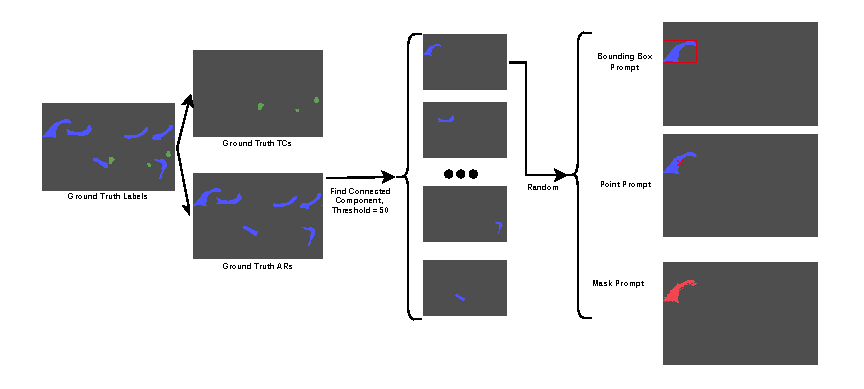
\includegraphics[width=1\textwidth]{graphics/approach/prompt_pipeline-1.pdf}
    \makebox[\textwidth][c]{%
    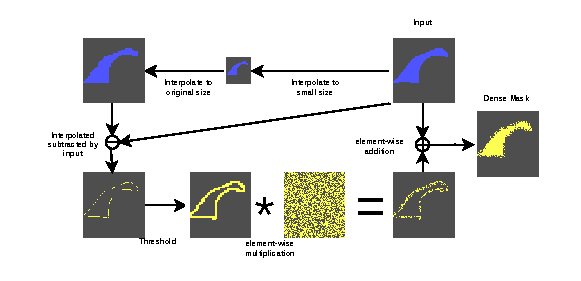
\includegraphics[width=1.2\textwidth]{graphics/approach/noisy_mask.pdf}
}
\vspace{-2em}
    \caption{Create Noisy Mask Prompts}
    \label{fig:noisy_mask_generation}
\end{figure}


% \begin{figure}[!h]
% \centering
% \vspace{-3em} 
% % Top Image
% % \begin{center}
% %     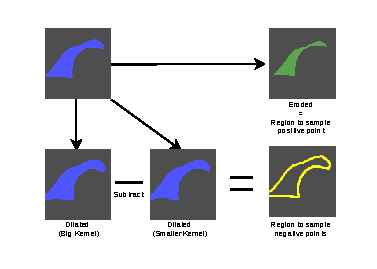
\includegraphics[width=0.7\textwidth]{graphics/approach/point_prompt.pdf}
% %     \caption{Sampling Negative and Positive Point Prompts}
% %     \label{fig:point_prompt_generation}
% % \end{center}
% \vspace{-3em} % Adds a small vertical gap between the two plots
% % Bottom Image
% \begin{center}
%     % \makebox[\textwidth][c]{%
%     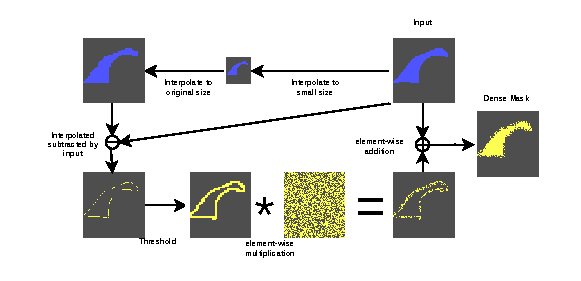
\includegraphics[width=1\textwidth]{graphics/approach/noisy_mask.pdf}
%     \caption{Create Noisy Mask Prompts}
%     \label{fig:noisy_mask_generation}
% \end{center}

% \caption{Prompt Generating Process}


% \end{figure}